\documentclass[areasetadvanced]{scrartcl}

\usepackage[utf8]{inputenc}
\usepackage[T2A]{fontenc}
\usepackage[english,russian]{babel}
\usepackage{dsfont}
\usepackage[footskip=1cm,left=25mm, right=15mm, top=20mm, bottom=20mm]{geometry}
\usepackage{setspace}
\usepackage{amsmath, amssymb}  % Объединено в одну строку
\usepackage{graphicx}
\usepackage{tikz}
\usetikzlibrary{arrows.meta}
\usepackage{float}
\usepackage{dashrule}
\usepackage{fancyhdr} % оформление отчёта
\usepackage{hyperref} % оформление отчёта
\usepackage{parskip}
\usepackage{textcomp, enumitem}
\usepackage{indentfirst}
\usepackage{graphicx}
\usepackage{algorithm}
\usepackage{algpseudocode}
\usepackage{array}  % Для использования команды m{}
\usepackage{geometry}
\usepackage{afterpage}
\usepackage{minted}
\setcounter{secnumdepth}{3}  % Включает нумерацию для subsubsection
\setcounter{tocdepth}{3}     % Включает subsubsection в содержание
\usepackage{listings} % Если используете listings

\tikzstyle{block} = [rectangle, rounded corners, minimum width=3cm, minimum height=1cm, text centered, draw=black, fill=lightgray]

\setkomafont{sectioning}{\normalfont\bfseries} % для заголовков разделов и подразделов
\setkomafont{section}{\normalfont\Large\bfseries}
\setkomafont{subsection}{\normalfont\large\bfseries}
\setkomafont{subsubsection}{\normalfont\large\bfseries}
\setkomafont{paragraph}{\normalfont\large\bfseries} % для заголовков параграфов (если они есть)

\lstset{
  language=Haskell,
  basicstyle=\ttfamily\small,
  keywordstyle=\color{blue}\bfseries,
  stringstyle=\color{red},
  commentstyle=\color{green!70!black},
  numbers=left,
  numberstyle=\tiny,
  stepnumber=1,
  numbersep=10pt,
  showstringspaces=false,
  breaklines=true,
  frame=single
}

\setcounter{tocdepth}{2}
\begin{document}
	\thispagestyle{empty}
	\begin{center}
		\large{МИНОБРНАУКИ РОССИИ} \par
		\vspace{0.3cm}
		\normalsize
		{ФЕДЕРАЛЬНОЕ ГОСУДАРСТВЕННОЕ АВТОНОМНОЕ ОБРАЗОВАТЕЛЬНОЕ УЧРЕЖДЕНИЕ ВЫСШЕГО ОБРАЗОВАНИЯ} \par
		\vspace{0.3cm}
		\textbf{\guillemotleft САНКТ-ПЕТЕРБУРГСКИЙ ПОЛИТЕХНИЧЕСКИЙ}
		\textbf{УНИВЕРСИТЕТ ПЕТРА ВЕЛИКОГО\guillemotright} \par
		\vspace{0.3cm}
		{Институт компьютерных наук и кибербезопасности}\par
		{Высшая школа технологий искусственного интеллекта}\par
	\end{center}
	\vfill
	\begin{center}
		{\large Отчёт по дисциплине \guillemotleft Математическая статистика\guillemotright}\par
		{\huge   \textbf{ИДЗ №2}
		
		\guillemotleft Оценивание параметра\guillemotright}\par
            {\huge Вариант \textbf{№25}}
         
	\end{center}
	\vfill
	\begin{flushleft}
		Студент: \hspace{1.8cm} \rule[0pt]{2.5cm}{0.5pt}\hfill Салимли Айзек Мухтар Оглы\par
		\vspace{1.5cm}
		Преподаватель: \hspace{0.55cm} \rule[0pt]{2.5cm}{0.5pt}\hfill Малов Сергей Васильевич
	\end{flushleft}
	\vspace{0.5cm}
	\begin{flushright}
		\guillemotleft \rule[0pt]{0.8cm}{0.5pt}\guillemotright \rule[0pt]{2cm}{0.5pt} 20\rule[0pt]{0.5cm}{0.5pt} г.
	\end{flushright}
	\vfill
	\begin{center}
		Санкт-Петербург, 2025
	\end{center}
	\newpage
	\tableofcontents
	\newpage
\section*{Введение}
	\addcontentsline{toc}{section}{Введение}
В отчете, решения задач №1, №2, №3.

\newpage
\section{Задача 1} 
Построить оценку максимального правдоподобия параметра $\theta = \sqrt{a}$ по выборке $X_1, \dots, X_n$ из распределения с плотностью:
\[
p(x;\theta) = 2a^{2}x \cdot \mathds{1}_{x \in [0, 1/a]},
\]
где $\mathds{1}$ - индикаторная функция.
\subsection{Решение}
\begin{itemize}
	\item Выборка $X_1, \dots, X_n$
	\item $\theta = \sqrt{a} \Longrightarrow a = \theta^2$
	\item $p(x, \theta) = 2a^{2}x\mathds{1}_{x\in[0,1/a]}$ = $2\theta^{4}x\mathds{1}_{x \in [0,1/\theta^{2}]}$ 
\end{itemize}
Функиця правдоподобия:
$L(X,\theta) = \prod_{i=1}^{n} 2 \theta^{4} x_i \mathds{1}_{x_i\in[0,1/\theta^2]} \textcircled{=} \triangle$ 


$\triangle:$
\begin{enumerate}
	\item $x_i \leq 1/\theta^2 \Longrightarrow \max(x_i) \leq 1/\theta^2$
	\item $X_{(n)} = \max(X_i)$ - порядковая статистика.
\end{enumerate}
\[
\textcircled{=} \quad
2^n \theta^{4n}\prod_{i=1}^{n}x_i \mathds{1}_{x_{(n)}\leq1/\theta^2} 
= 
\underbrace{2^n \theta^{4n} \mathds{1}_{x_{(n)}\leq 1/\theta^2}}_{\textstyle g_\theta(T(x))} 
\cdot 
\underbrace{\prod_{i=1}^{n}x_i}_{\textstyle h(x)}
\]

МДС: $T=X_{(n)}$
\[
\left\{
\begin{array}{l}
2^n \theta^{4n} \prod_{i=1}^{n} x_i \\
x_{(n)} \leq 1/\theta^2
\end{array}
\right\}
\quad
\rightarrow
\quad
\max
\]
\begin{enumerate}
	\item \[ \begin{cases}
		X_{(n)} \leq 1/\theta^2
		\theta^2 \leq 1/X_{(n)} 
		\theta \leq \frac{1}{\sqrt{X_{(n)}}}
	\end{cases} 
	\]
	\item \[ lL(x, \theta) = n\ln2 + 4n\ln\theta + \sum_{i=1}^{n}\ln{x_i} \]
	\item \[
		\frac{\partial{lL(x,\theta)}}{\partial{\theta}} = \frac{4n}{\theta}
		\Longrightarrow \theta > 0
		\]
		\subitem Производная положительна и монотонно возрастает \( (4n \ln{\theta}) \), максимум на верхней границе.
		
		
\end{enumerate}
Ответ: \[ \hat{\theta} = \frac{1}{\sqrt{x_{(n)}}}\]
\newpage
\section{Задача 2}
Построить оценку параметра $ \theta = b^2$ по выборке $X_1, \dots, X_n$ из распределения с плотностью:
\[
p_\theta(x) = \frac{x^{p-1} e^{-x/b}}{b^{p}\Gamma(p)}\mathds{1}_{x > 0}
\]

\subsection{Решение}

\begin{itemize}
    \item Выборка: $X_1, \dots, X_n$
    \item $\theta = b^2 \Rightarrow b = \sqrt{\theta}$
    \item Подставим в плотность: 
    \[
    \frac{x^{p-1}e^{-x/b}}{b^p \Gamma(p)} = \frac{x^{p-1}e^{-x/\sqrt{\theta}}}{\theta^{p/2} \Gamma(p)}
    \]
\end{itemize}

\[
L(x,\theta) = \prod_{i=1}^{n} \frac{x_{i}^{p-1} e^{-x_i/\sqrt{\theta}}}{\theta^{p/2} \Gamma(p)}
= \frac{1}{\theta^{np/2} [\Gamma(p)]^n} \prod_{i=1}^{n} x_i^{p-1} \cdot e^{-\frac{1}{\sqrt{\theta}} \sum_{i=1}^{n} x_i}
\]
\begin{enumerate}
    \item \( g(T(x)) = \dfrac{e^{-\frac{1}{\sqrt{\theta}} \sum\limits_{i=1}^{n} x_i}}{\theta^{\frac{np}{2}}} \)
    
    \item \( L(x) = \prod\limits_{i=1}^{n} x_i^{p-1} \cdot \dfrac{1}{[\Gamma(p)]^n} \)
\end{enumerate}

\textbf{МДС:} \( T(x) = \sum\limits_{i=1}^{n} x_i \)

\[
\ell(x, \theta) = (p - 1) \sum_{i=1}^{n} \ln x_i - \frac{1}{\sqrt{\theta}} \sum_{i=1}^{n} x_i - \frac{np}{2} \ln \theta - n \ln \Gamma(p)
\]

\vspace{1em}

\[
\frac{\partial \ell(x, \theta)}{\partial \theta} = \frac{1}{2 \theta \sqrt{\theta}} \sum_{i=1}^{n} x_i - \frac{np}{2\theta}
\]

\[
\frac{1}{2\theta} \left( \frac{\sum\limits_{i=1}^{n} x_i}{\sqrt{\theta}} - np \right) = 0
\]

\[
\sqrt{\theta} = \frac{1}{np} \sum_{i=1}^{n} x_i 
\]

\[
\hat{\theta} = \left( \frac{\bar{x}}{p} \right)^2 \quad \text{— ОМП}
\]

\textbf{Ответ:} \( \hat{\theta} = \left( \dfrac{\bar{x}}{p} \right)^2 \quad \text{— ОМП} \)
\newpage
\section{Задача 3}
Даны две независимые выборки \( X_1, \ldots, X_n \) из \( \mathcal{N}(a, 1) \) и \( Y_1, \ldots, Y_m \) из \( \mathcal{N}(b, 8) \). Построить доверительный интервал для \( 3a - 2b \).

\subsection{Решение}
Независимые выборки:
\[
\left[
\begin{array}{l}
X_1, \dots, X_n \sim \mathcal{N}(a, 1) \\
Y_1, \dots, Y_m \sim \mathcal{N}(b, 8)
\end{array}
\right]
\]
% ↑ Здесь исправлено \right. на \right], чтобы закрыть скобку

По лемме Фишера:
\begin{itemize}
	\item $\sqrt{n}\dfrac{\bar{x}-1}{1} \sim \mathcal{N}(0,1)$
	\subitem $\dfrac{n(S_x)^2}{1} \sim \chi^2_{n-1}$
	\item $\sqrt{m}\dfrac{\bar{y}-1}{\sqrt{8}} \sim \mathcal{N}(0,1)$
\end{itemize}

\begin{enumerate}
	\item $\bar{x}-a \sim \mathcal{N}(0,1)$
	\subitem $3\bar{x}-3a \sim \mathcal{N}(0, 9/n)$
	\item $\bar{y}-b \sim \mathcal{N}(0,1/m)$
	\subitem $2\bar{y}-2b \sim \mathcal{N}(0, 32/m)$
	\subitem \[
	3\bar{x}-3a - 2\bar{y}+2b = (3\bar{x}-2\bar{y}) - (3a-2b) \sim \mathcal{N}\left(0, \frac{9}{n} + \frac{32}{m}\right) \text{, т.е. } \sim \mathcal{N}\left(0, \frac{9m+32n}{nm}\right)
	\]
	\subitem \[ \frac{(3\bar{x} - 2\bar{y} - \theta)}{\sqrt{\frac{9m+32n}{nm}}} \sim \mathcal{N}(0,1) \]
	\item $\dfrac{n(S_x)^2}{1} + \dfrac{m(S_y)^2}{8} \sim \chi^2_{n+m-2}$
\end{enumerate}
$$ p_\theta\Bigl(
 -X_\alpha 
 \;\le\; 
 \frac{(3\bar{x} - 2\bar{y} - \theta)\,C_{(n,m)}}{\sqrt{(nS_x)^2 + \frac{(mS_y)^2}{8}}}
 \;\le\;
 X_\alpha
\Bigr)
\;=\;
1-\alpha $$

\newpage

$ 
\Longrightarrow
\quad
p_\theta\Bigl(
  3\bar{x} - 2\bar{y}
  \;-\;
  X_\alpha
  \,\frac{\sqrt{(nS_x)^2 + \frac{(mS_y)^2}{8}}}{C_{n,m}}
  \;\le\;
  \theta
  \;\le\;
  3\bar{x} - 2\bar{y}
  \;+\;
  X_\alpha
  \,\frac{\sqrt{(nS_x)^2 + \frac{(mS_y)^2}{8}}}{C_{n,m}}
\Bigr)
\;=\;
1-\alpha
\;\Longrightarrow\;
\frac{
  \dfrac{3\bar{x}-2\bar{y}-\theta}{\sqrt{\frac{9m+32n}{nm}}}
}{
  \sqrt{
    \dfrac{1}{n+m-2}
    \Bigl(
      \dfrac{n(S_x)^2}{1}
      + \dfrac{m(S_y)^2}{8}
    \Bigr)
  }
}
\;\sim\;
t_{n+m-2}.
$
\[
\sqrt{\frac{9m+32n}{nm(n+m-2)}
      \Bigl((nS_x)^2 + \frac{(mS_y)^2}{8}\Bigr)}
\frac{3\bar{x} - 2\bar{y}-\theta}{\sqrt{(nS_x)^2 + \frac{(mS_y)^2}{8}}}
\sqrt{\frac{nm(n+m-2)}{9m+32n}}
\sim S_{n+m-2}
\]
% ↑ Внутри корня добавлены скобки \Bigl(...\Bigr), чтобы Latex корректно понимал выражение

\[
p_\theta (-X_\alpha \leq \frac{(3\bar{x} - 2\bar{y} - \theta)C_{(n,m)}}{\sqrt{(nS_x)^2 + \frac{(mS_y)^2}{8}}} \leq X_\alpha) = 1-\alpha
\Longrightarrow 
\]
\[
p_\theta(3\bar{x} - 2\bar{y} - X_\alpha \frac{\sqrt{(nS_x)^2 + \frac{(mS_y)^2}{8}}}{C_{n,m}} \leq \theta \leq 3\bar{x}-2\bar{y}+X_\alpha \frac{\sqrt{(nS_x)^2 + \frac{(mS_y)^2}{8}}}{C_{n,m}}) = 1-\alpha
\]
Ответ: \[
(3\bar{x} - 2\bar{y} - X_\alpha \frac{\sqrt{(nS_x)^2 + \frac{(mS_y)^2}{8}}}{C_{n,m}}
\;\;\leq\;\;
\theta
\;\;\leq\;\;
3\bar{x}-2\bar{y} + X_\alpha \frac{\sqrt{(nS_x)^2 + \frac{(mS_y)^2}{8}}}{C_{n,m}}
)
\]


\newpage
\section*{Заключеине}
\addcontentsline{toc}{section}{Заключение}
\begin{enumerate}
	\item Ответ: \[ \hat{\theta} = \frac{1}{\sqrt{x_{(n)}}}\]
	\item Ответ: \[
\hat{\theta} = \left( \frac{\bar{x}}{p} \right)^2 \quad \text{— ОМП}
\]
	\item Ответ:\[
(3\bar{x} - 2\bar{y} - X_\alpha \frac{\sqrt{(nS_x)^2 + \frac{(mS_y)^2}{8}}}{C_{n,m}}
\;\;\leq\;\;
\theta
\;\;\leq\;\;
3\bar{x}-2\bar{y}+X_\alpha \frac{\sqrt{(nS_x)^2 + \frac{(mS_y)^2}{8}}}{C_{n,m}}
)
\]
\end{enumerate}
\newpage
\section*{Приложение A}
\addcontentsline{toc}{section}{Приложение А}
\subsection*{Фото: Решение задачи 1}
\begin{figure}[H]
    \centering
    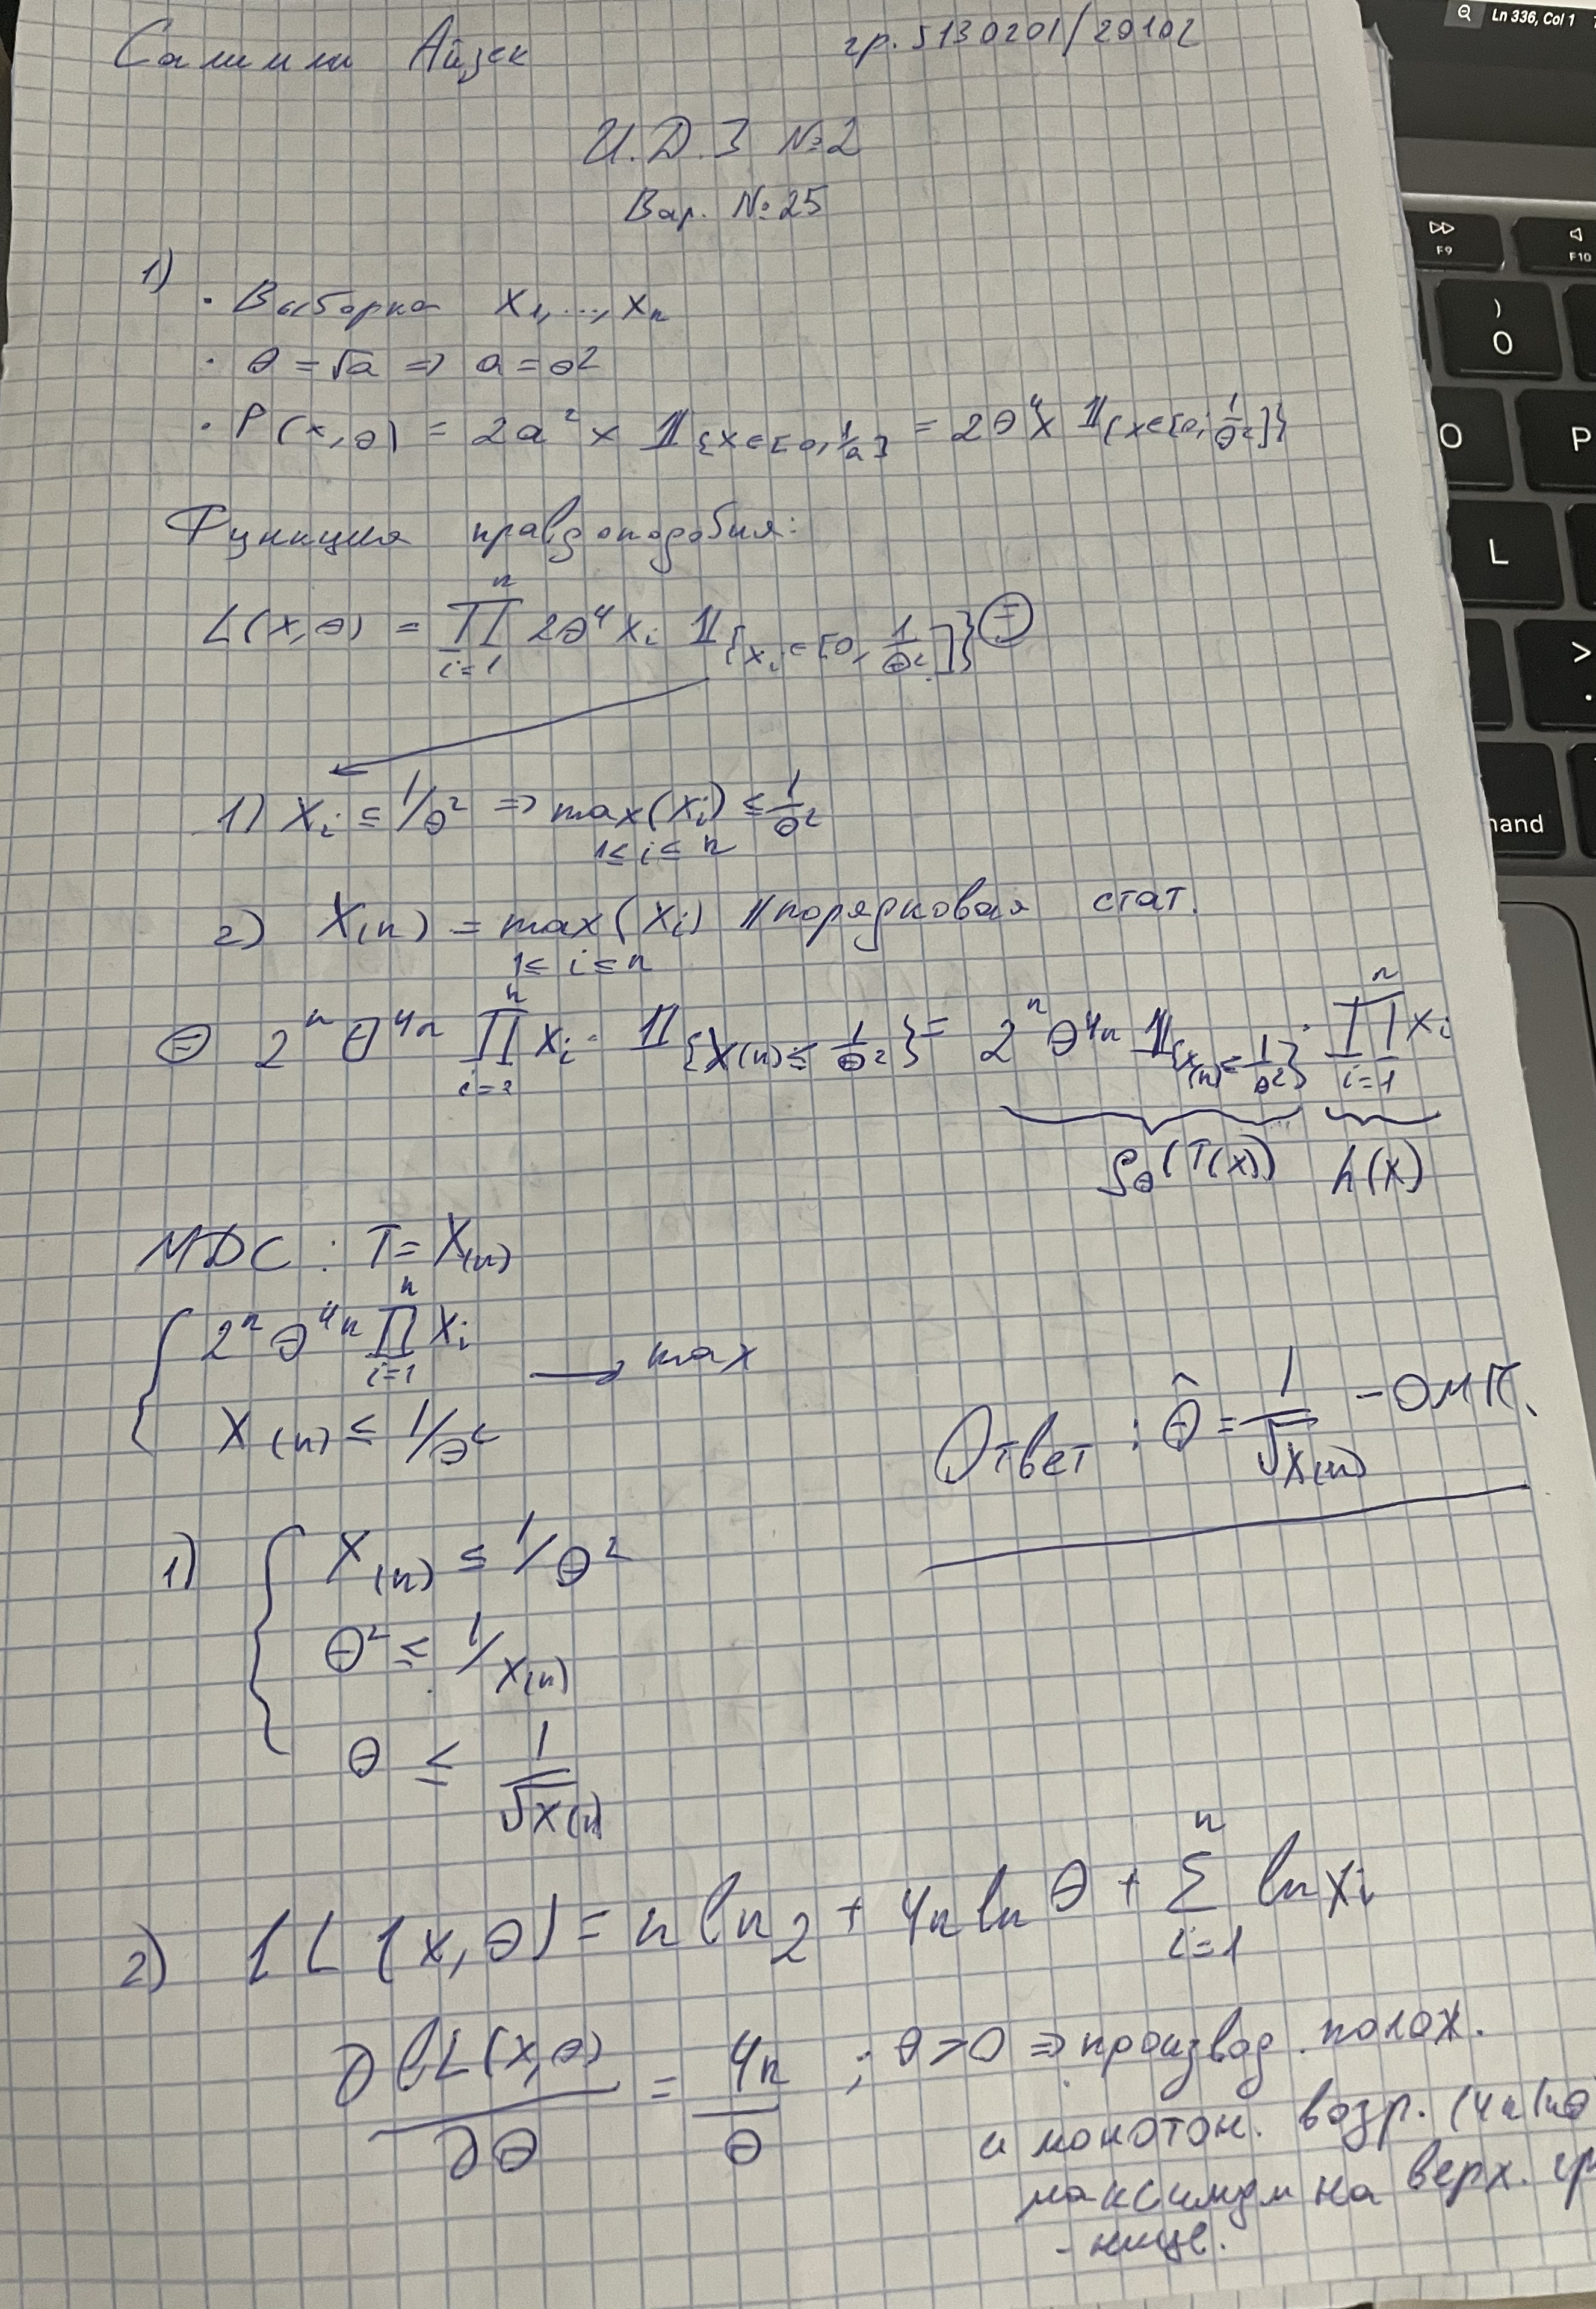
\includegraphics[width=0.7\textwidth]{1.png}
    \caption{Задача 1}
    \label{fig:syntdiag}
\end{figure}
\newpage
\subsection*{Фото: Решение задачи 2}
\begin{figure}[H]
    \centering
    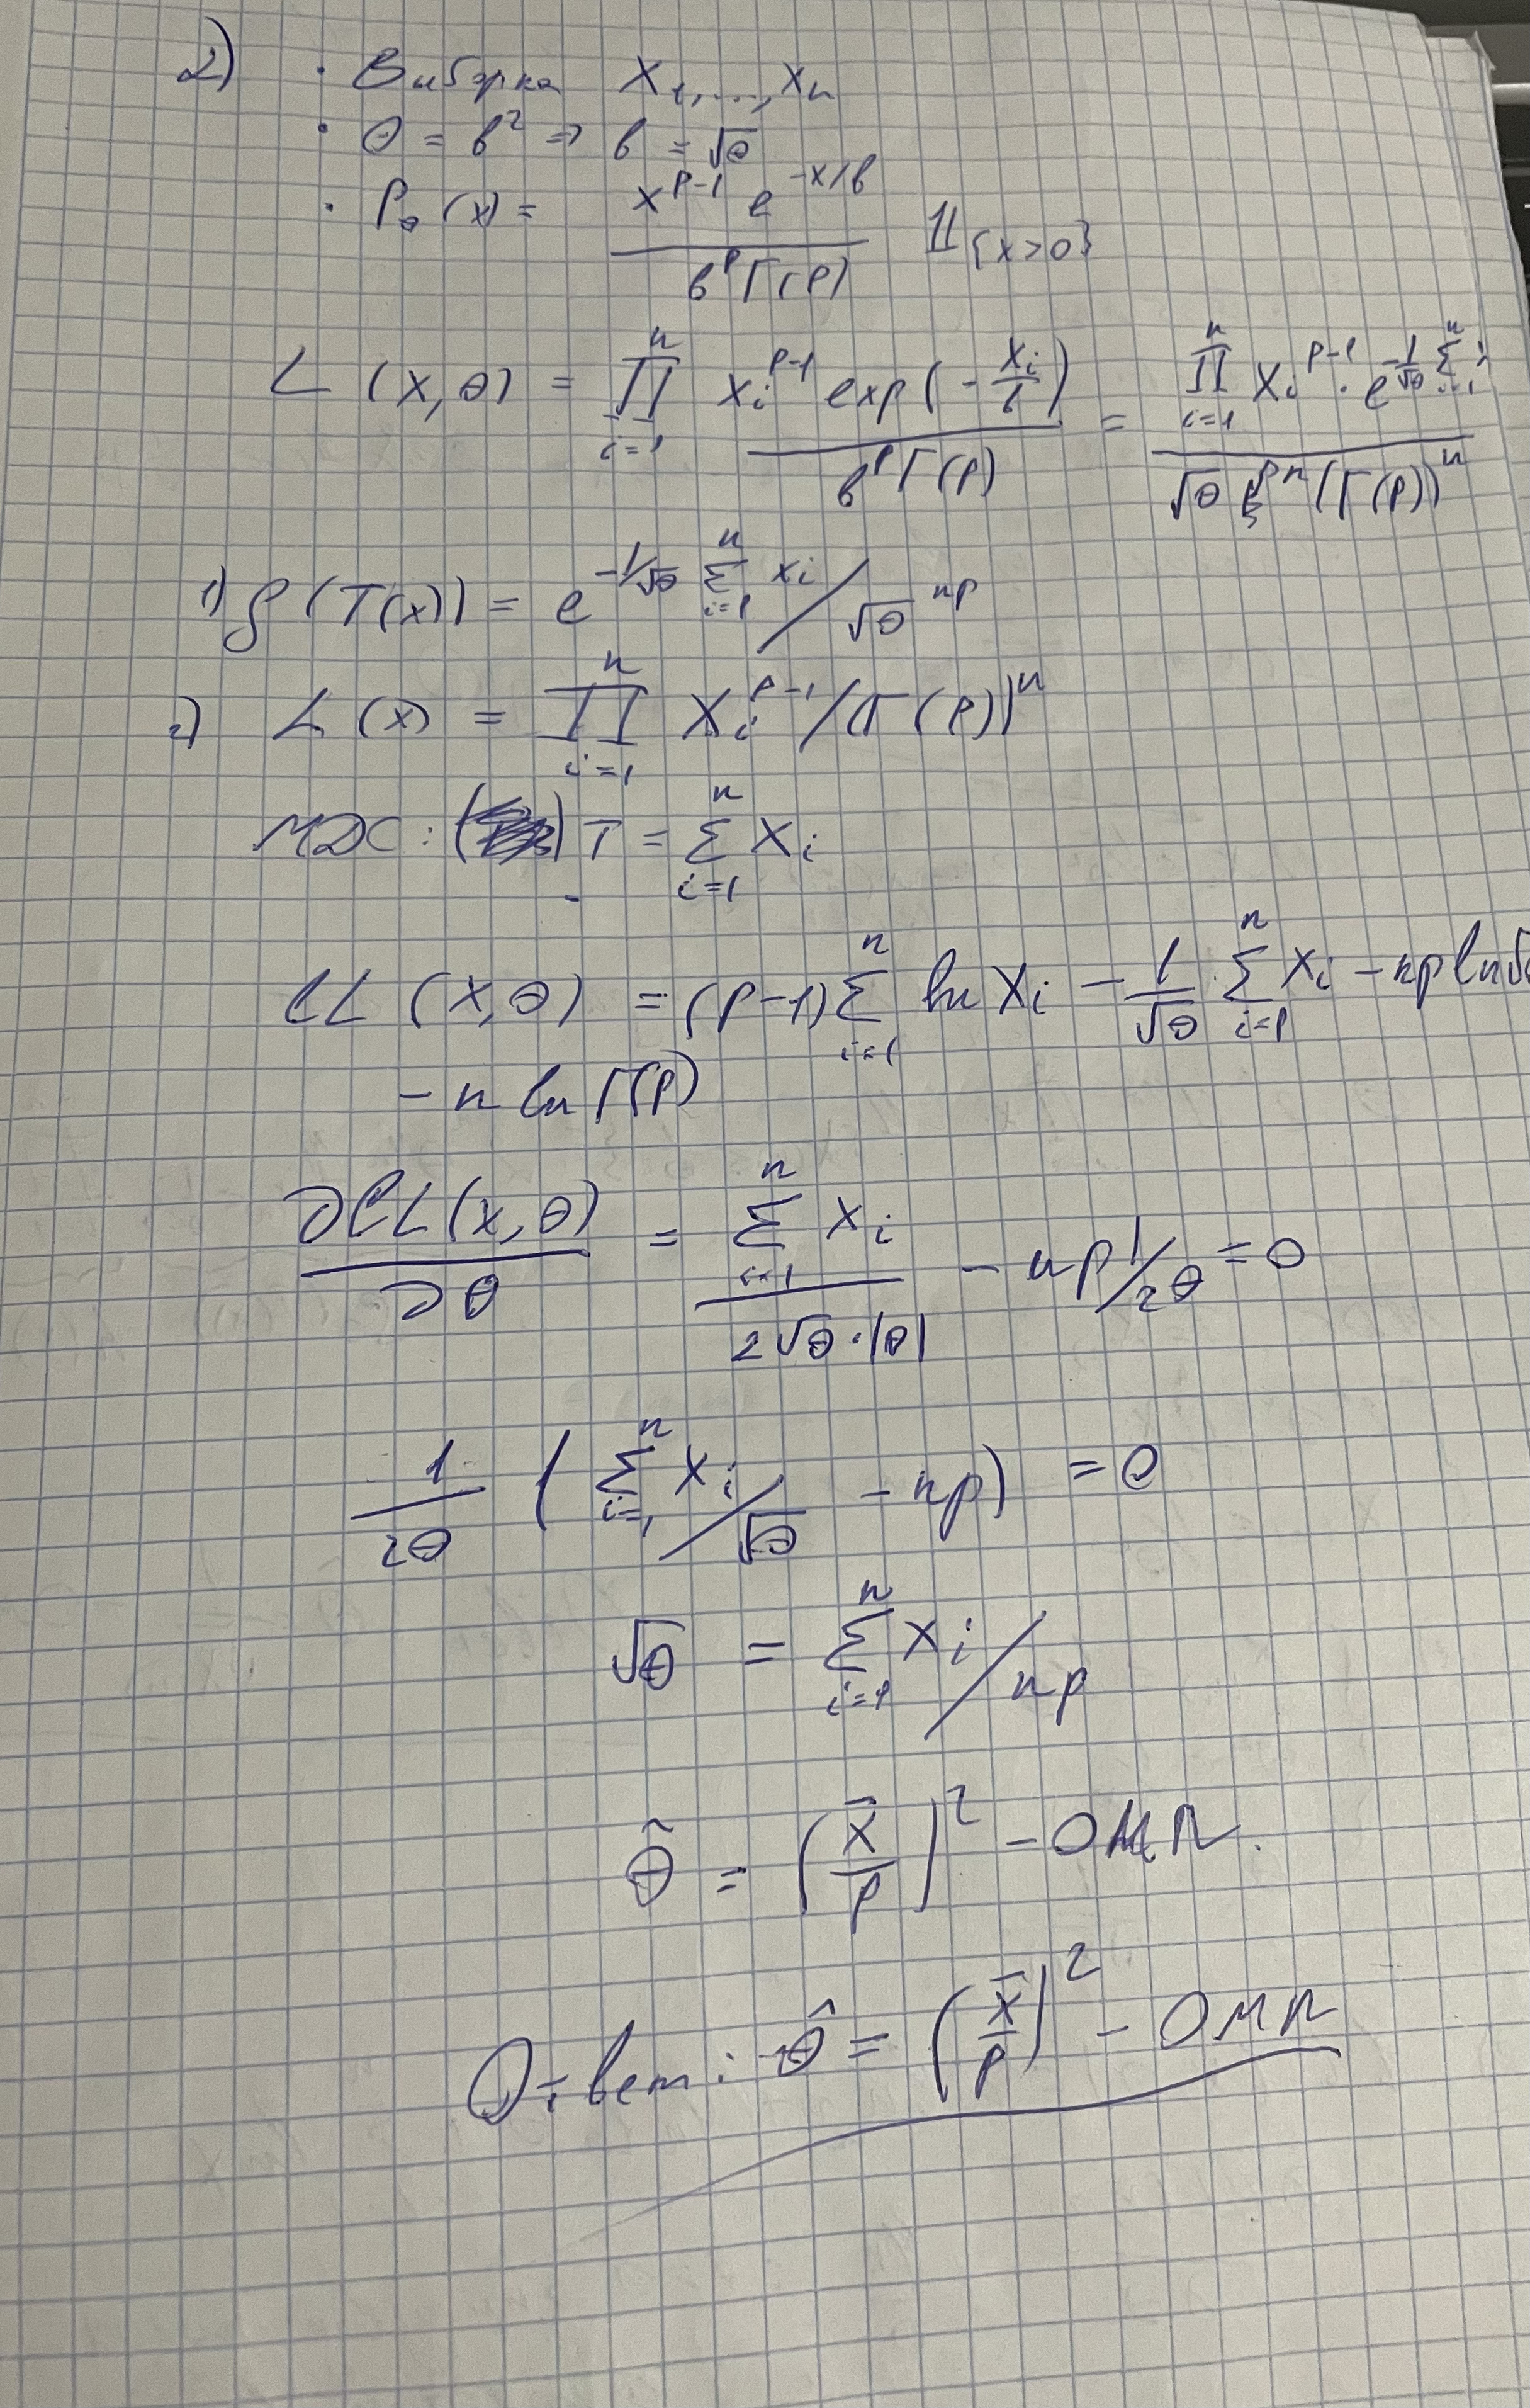
\includegraphics[width=0.7\textwidth]{2.png}
    \caption{Задача 2}
    \label{fig:syntdiag}
\end{figure}
\newpage
\subsection*{Фото: Решение задачи 3}
\begin{figure}[H]
    \centering
    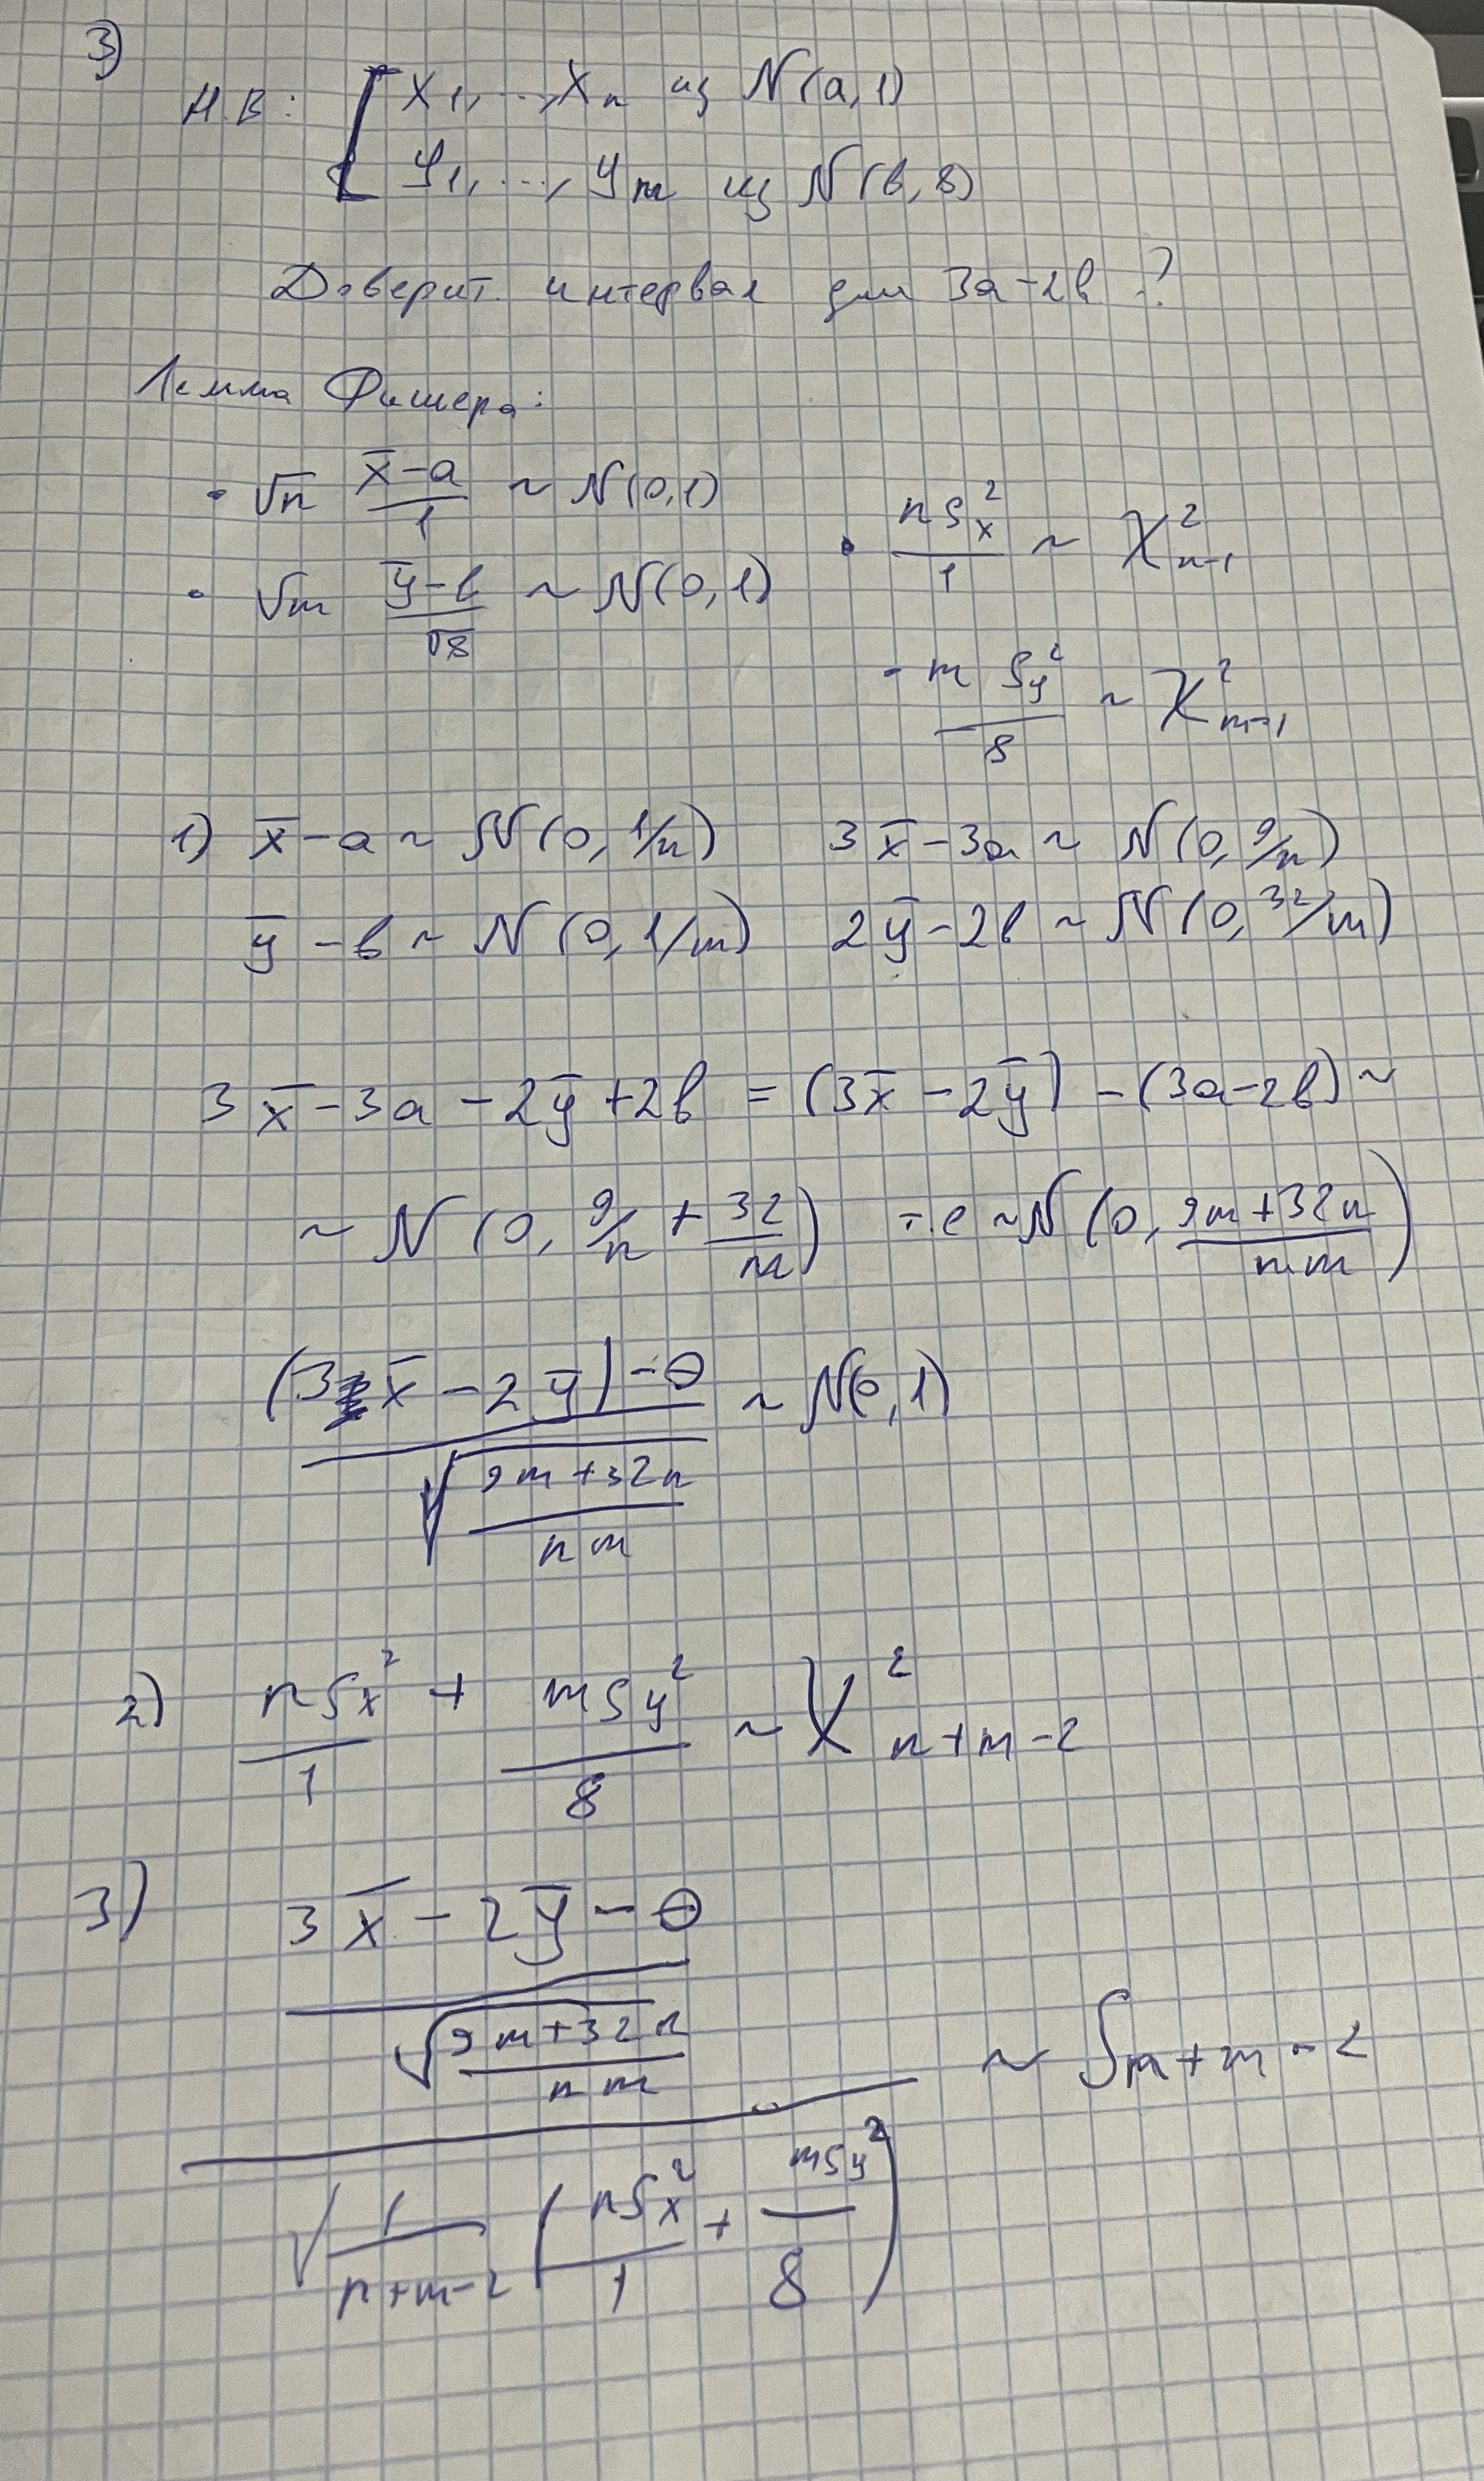
\includegraphics[width=0.7\textwidth]{3.png}
    \caption{Задача 3 начало}
    \label{fig:syntdiag}
\end{figure}
\newpage
\begin{figure}[H]
    \centering
    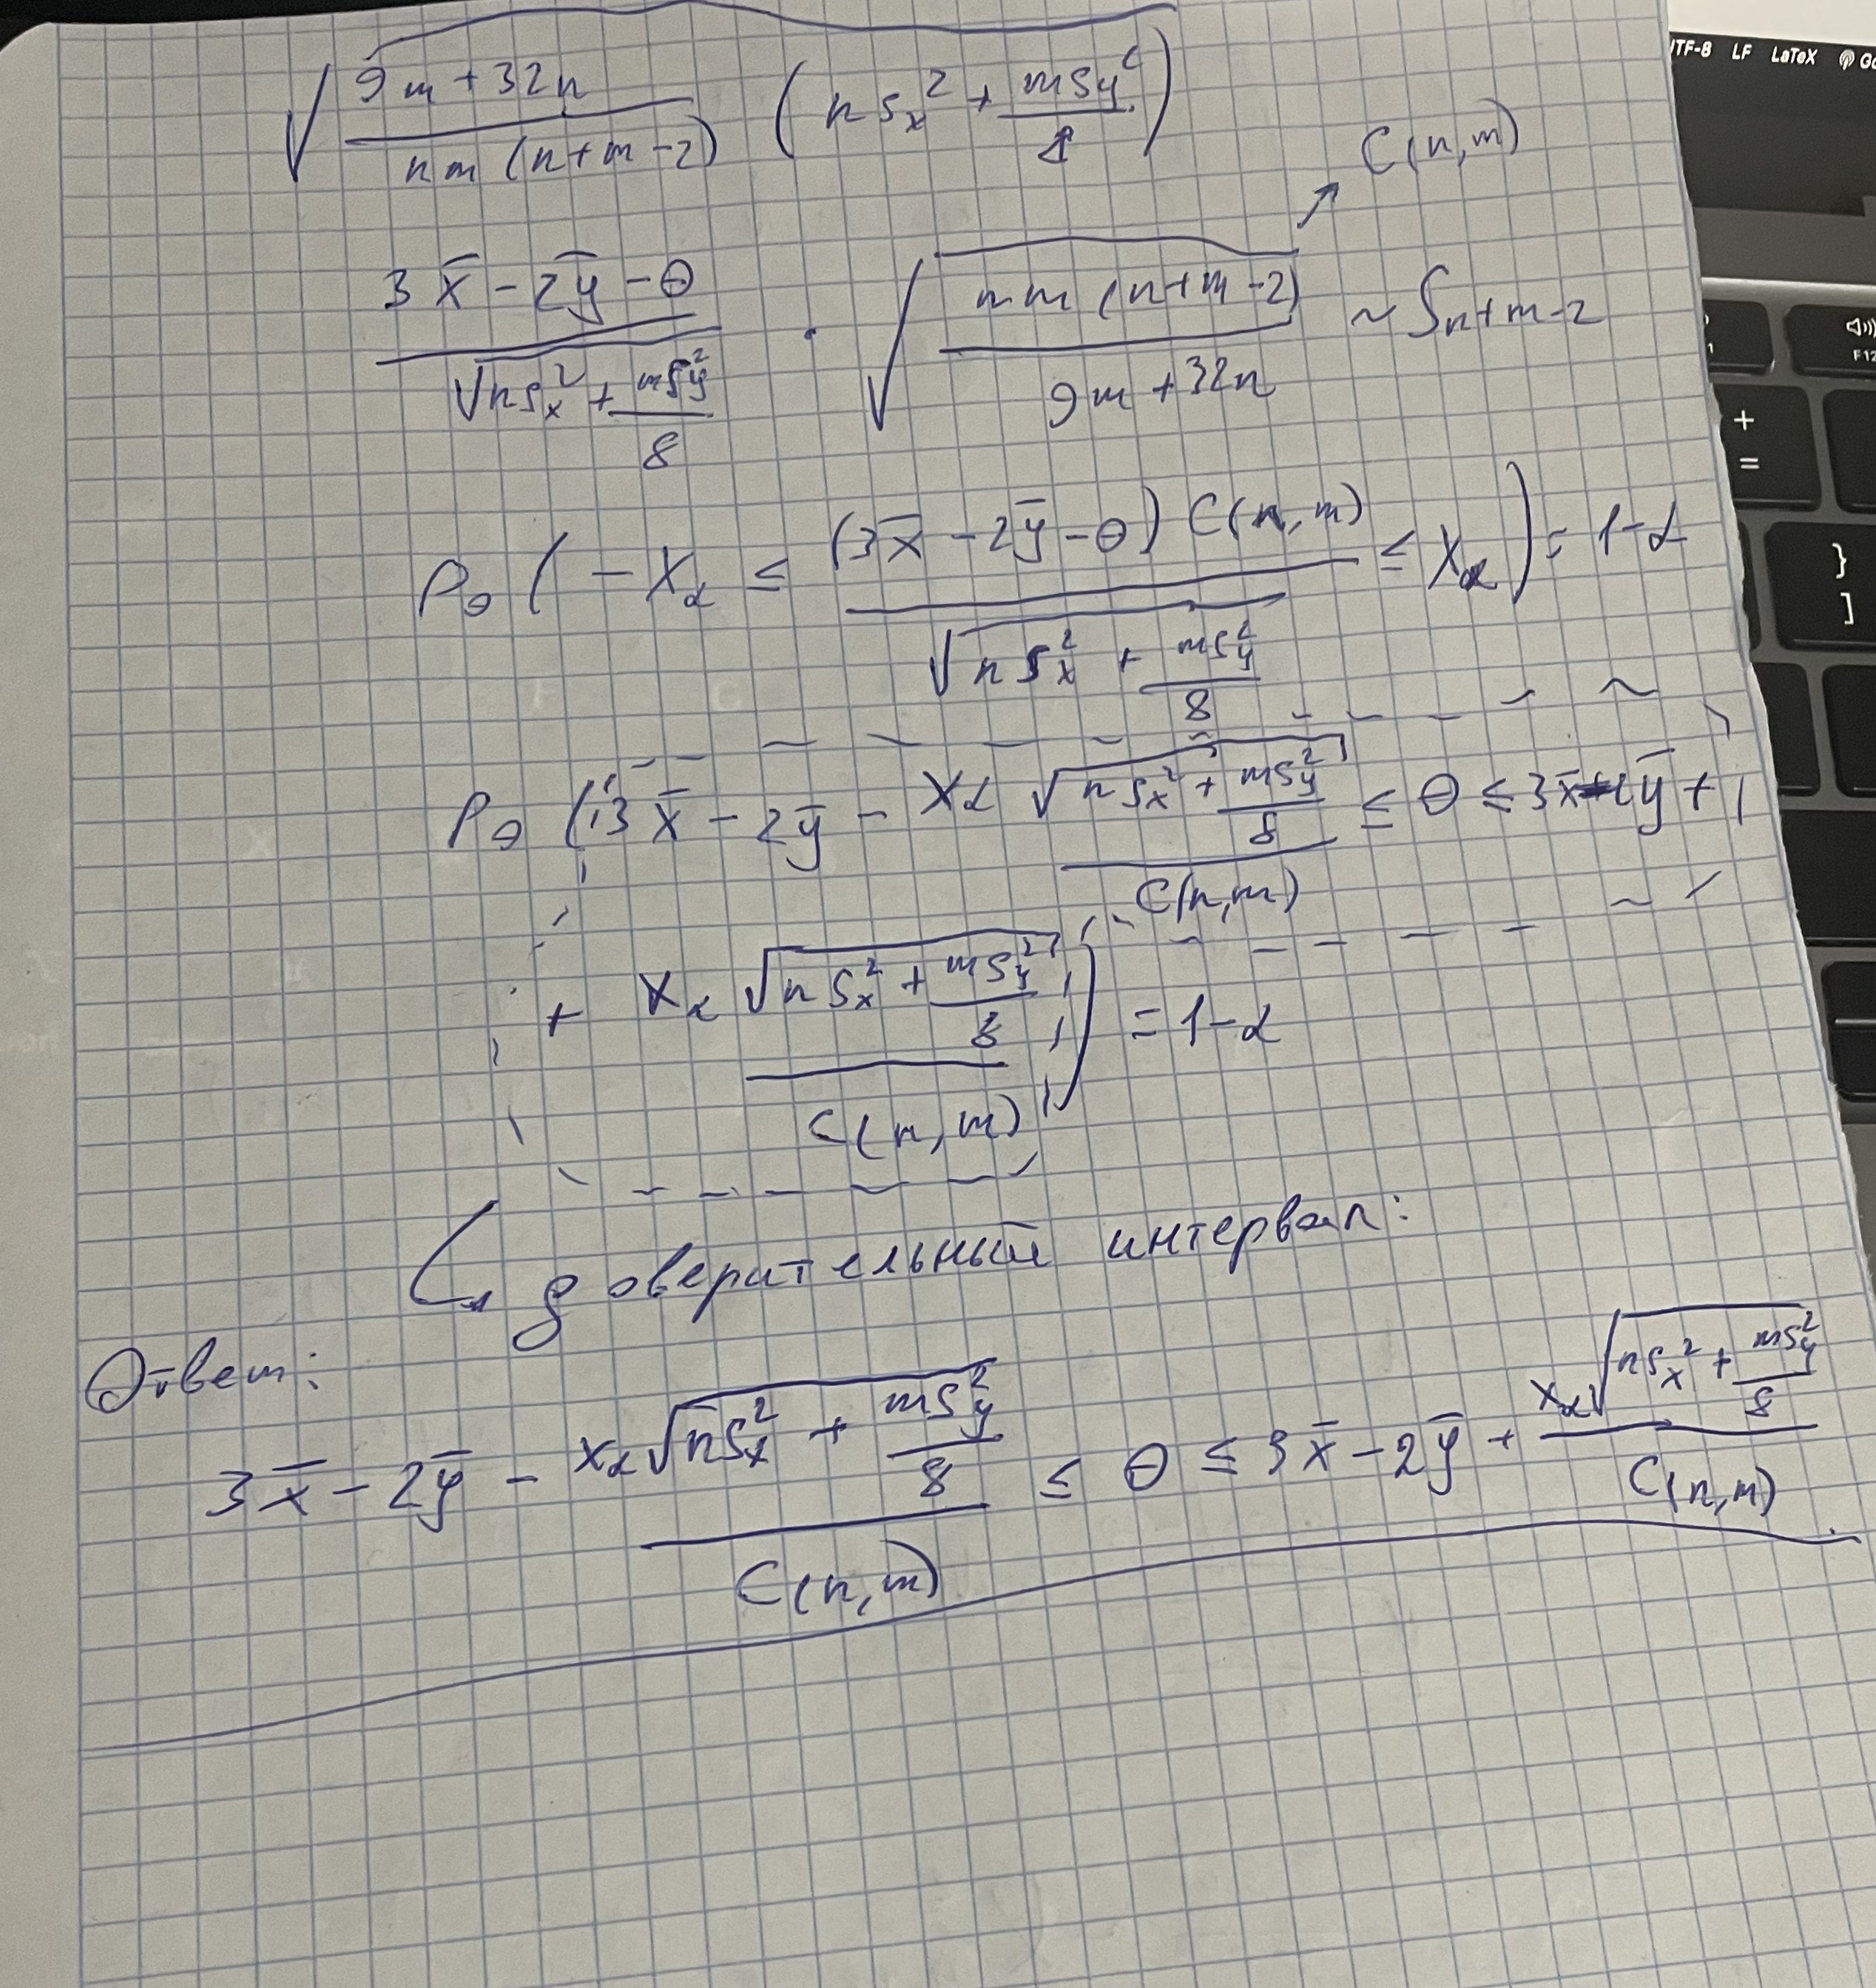
\includegraphics[width=0.7\textwidth]{4.png}
    \caption{Задача 3 продолжение}
    \label{fig:syntdiag}
\end{figure}
\end{document}